
\chapter{\label{cha:res-bg}Research Background}

\section{Edge Labelled Graph}
A graph $G$ can be modelled as a pair $(V, E)$, where $V$ is a finite set of nodes and $E$ is a finite set of edges connecting pairs of nodes. In some cases, the edges are labelled with strings from a finite set of symbols, representing the attribute value from starting node to ending node. The symbols are drawn from some finite alphabet $\Sigma$; Hence a labelled directed graph could be modelled as 
$(V,E,\Sigma)$, where $E\subseteq V\times\Sigma\times V$.\\
\section{Graph Database}
In the context of graph databases, we focus on permanent storage and query evaluation at the same time, which is why graph processing framework such as Pregel or Trinity are not taken into consideration here.
\subsection{Vertical Scaling Graph Database}
\textbf{Neo4j}\cite{neo4j} is one of the most popular graph databases, which provides full ACID transaction support, indexing, a web UI for graph visualisation and supports diverse query languages such as Cypher, Gremlin and even SPARQL. Neo4j uses a custom disk-based native storage engine. Neo4j believes vertical scaling could solve most scaling problems of graph databases, so Neo4j graph database can only be deployed on a single machine. With Cypher, we can query Neo4j with a subset of RPQ and write queries like this: MATCH $ n-[?:KNOWS*..5]->m$, which will find out all pairs $(n,m)$ where there are paths between them consisting of at most 5 "KNOWS" labels.\\

\noindent\textbf{Sparksee}\cite{sparksee} is a graph database written in C++ and provides API in diverse programming languages in Python, C++, .Net, Java, Objective-C, etc. It can be deployed on Linux, Windows, MacOSX and even mobile systems such as Android or IOS. Sparksee splits graphs into small structures and caches the most significant parts. It also has mechanisms for indexing nodes, edges and attributes. It supports concurrent query processing, but not distributed storage and querying.

\subsection{Distributed Graph Database}

\textbf{Titan}\cite{titan} is one of the most popular distributed graph databases, which can use different storage back-ends such as Cassandra, HBase or BerkeleyDB. Although Titan 1.0 released in September, 2015 has implemented the latest version of the popular Apache Gremlin query language, from which it's possible to traverse graphs by the Spark-gremlin connector in a distributed way, the project is still far from maturity and under community testing. Furthermore, graph analytics and global breadth-first execution of Gremlin queries is executed by Apache Spark through the Cassandra-Spark connector, which is similar to our own system architecture.\\


\noindent\textbf{imGraph}\cite{imgraph} is a distributed in-memory graph database, which provides distributed memory storage and distributed processing features, however, it doesn't support regular path queries and huge graphs cannot always fit in memory.\\

\noindent\textbf{OrientDB}\cite{orientdb} is a database of hybrid Document-Graph data models. In order to achieve higher scalability, it adopts Multi-Master + Sharded architecture: all the servers are masters. Similar to Neo4j, OrientDB has its own query language OrientDB SQL, which is quite similar to SQL syntactically.\\

\noindent\textbf{GBase}\cite{GBase} is a platform conceived to handle large static graphs that uses the sparse adjacency matrix format as data model. The graph data is stored and indexed by storing compressed blocks in distributed storage such as HDFS. It does not support RPQ and cannot work for dynamic graphs.\\

\noindent\textbf{Infinitegraph}\cite{infinitegraph} is an enterprise distributed graph database implemented in Java. In its graph data model, edge is the first-class entity with an identity independent of the vertices it connects. Infinitegraph supports full ACID, and provides path pattern matching feature.\\

To summarize, I extend the table which compares graph databases in imgraph paper\cite{imgraph} to following table 2.1.
\begin{table}[h!]
\scriptsize
\def\arraystretch{1.5}
\centering
\caption{Graph Database Overview}
\label{graph-database-overview}
\begin{tabular}{|l|m{5em}|m{5em}|m{5em}|m{5em}|m{5em}|m{5em}|}
\hline
 & Native Graph Model & Distributed Storage & Distributed query processing & Transactions and index support & Support RPQ & License \\
\hline
Neo4j & Yes & No & No & Yes & Partially & Conditional \\
\hline
Sparksee & Yes & NO & NO & Yes & No & Free Research License \\
\hline
Titan & Yes & Yes & No & Yes & No & Free \\
\hline
imGraph & Yes & Yes & Yes & Yes & No & Free \\
\hline
OrientDB & Yes & Yes & Yes & Yes & No & Conditional \\
\hline
GBase & No & Yes & Yes & No & No & Free \\
\hline
Infinitegraph & Yes & Yes & Yes & Yes & No & Enterprise\\
\hline
\end{tabular}
\end{table}
\section{Regular Path Query Classes}
There are a variety of ways to define the classes for RPQ. For example, in Wood's work\cite{wood2012query}, RPQs are divided into four classes:
\begin{enumerate}
\item conjunctive queries (CQ)
\item regular path queries (RPQ)
\item conjunctive regular path queries (CRPQ), which is the combination of CQ and RPQ.
\item extended conjunctive regular path queries (ECRPQ).
\end{enumerate}
In the paper by Reutter et al. \cite{reutter2015regular}, he and his colleagues extend the expressiveness of RPQ. More categories are produced:
\begin{enumerate}
\item 2-way regular path queries (2RPQ), in which inverse labels are allowed.
\item conjunctive two-way regular path queries (C2RPQ)
\item nested two-way regular path queries (N2RPQ), where recursive variable is allowed in regular expression.
\item union of conjunctive two-way regular path queries (UC2RPQ), where we can perform unions, joins and projections over 2RPQs.
\item union of conjunctive nested two-way regular path queries (UCN2RPQ), where we can perform unions, joins and projections over N2RPQs. 
\end{enumerate}
In this thesis work, the query classes can be reduced by allowing inverse edges and nested variables in regular path query. For conjunctive regular path queries, we will stop at C2RPQ, which means calculating the intersection of results of 2RPQs.
\subsection{Regular Path Query}
Given a finite alphabet $\Sigma$, the regular expression over $\Sigma$ is defined by following grammar:
$$ n := \ \epsilon \ | \ a \ (a\in \Sigma) \ | \ a^- \ (a\in \Sigma) \ | \ n\ + \ n \ | \ n\ *\ n \ | \ n^* \  $$
The regular expression $n$ can be one of the following:
\begin{enumerate}
    \item Empty Expression.
    \item A label $a$ from $\Sigma$.
    \item The reverse of a label $a$ from $\Sigma$.
    \item The alternation of two regular expressions.
    \item The concatenation of two regular expressions.
    \item Zero or more recurrence of a regular expression.
\end{enumerate}
Furthermore, The semantic of regular path expression over a graph database $G=(V,E)$ can be defined as binary relation $[n]_G$ as follows:
$$[\epsilon]_G = \{(u,u) \ |u\in V\}$$
$$[a]_G = \{(u,v) \ |\ (u,a,v) \in E\}$$
$$[a^-]_G = \{ (u,v) \ |\ (v,a,u) \in E\}$$
$$[n_1\ +\ n_2]_G = [n_1]_G \ \cup \ [n_2]_G $$
$$[n_1\ *\ n_2]_G = [n_1]_G \ \circ \ [n_2]_G$$
$$[n^*]_G = [\epsilon]_G \ \cup \ [n]_G \ \cup \ [n*n]_G \ \cup \ [n*n*n]_G \ \cup \ ...   $$
where $[n_1]_G \ \circ \ [n_2]_G=\{ (u,v) | \ \exists w \ such \ that \ (u,w)\in [n_1]_G \ and \ (w,v) \in [n_2]_G \}$. By convention, we treat $[n^+]_G$ as $[n]_G*[n^*]_G.$
\subsection{Conjunctive Regular Path Query}
\subsubsection{Conjunctive Query}
For a set of node variables $\{ x_1,y_1,x_2,y_2,...,x_m,y_m \}$, the conjunctive query(CQ) Q over a finite alphabet $\Sigma$ is a query in the form:
$$ans(z_1,z_2,...,z_n) \leftarrow \cap_{i=1}^{m} (x_i,a_i,y_i)$$
where $m>0$, each $a_i \in \Sigma (1\leq i \leq m)$ and each $z_i$ is some $x_j$ or $y_j$ $(1\leq i \leq n,1\leq i \leq m)$. The semantics of CQs of this form is finding all node binding for all node variables in a graph. For example, a CQ for MATRIX graph could be:\\
$$ans(x,y)\leftarrow (x,LOVES,y),(x,KNOWS,y)$$
which return (Neo,Trinity) as it's the only pair that satisfies the node bindings for x and y.\\
The CQs are in some sense the simplest form of graph queries, the complexity of which is NP-complete as it's the same as the problem of subgraph homomorphism.
\subsubsection{Conjunctive Regular Path Query}
Conjunctive Regular Path Queries are similar to Conjunctive Query, except replacing symbol $a_i$ with a regular expression $r_i$. So a conjunctive regular path query(CRPQ) Q over $\Sigma$ is an expression of the form:
$$ans(z_1,z_2,...,z_n) \leftarrow \cap_{i=1}^{m} (x_i,r_i,y_i)$$
The example in previous section then could be:
$$ans(x,y)\leftarrow (x,LOVES,y),(x,KNOWS^*,y)$$
which still returns (Neo,Trinity) but with a larger result space for sub-query $(x,KNOWS^*,y)$.\\
Specifically, in this project we experiment with a sub-class of CRPQ:
$$ans(x,y) \leftarrow \cap_{i=1}^{m} (x,r_i,y)$$
which only contains two node variables, but more basic to experiment with. In section 5 Vertex-Signature Index Tree will be used to accelerate evaluation of the basic CRPQ problem.
\section{Evaluation of RPQ}
Breadth first search (BFS) is widely used while evaluating RPQ\cite{mendelzon1995finding}\cite{koschmieder2012regular}\cite{tung2013efficient}, and in order to search graphs efficiently, automata are often introduced into the process.
\subsection{Automata Based Search}
Regular path queries can be translated into an automata naturally by constructing a deterministic finite automation (DFA). For example, the regular path query $(LOVES|KNOWS^+)*CODED\_BY$ can be translated into automata in Figure ~\ref{fig:example-automata}.
\begin{figure}[h!]
  \caption{Example Automata}
  \label{fig:example-automata}
  \centering
    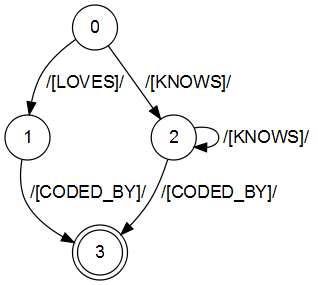
\includegraphics[width=0.5\textwidth]{img/automata-example}
\end{figure}
Now we try to match automata with the example graph (Figure ~\ref{fig:example-matrix}). The search is performed breadth-first by iterating through the graph and the query automata at the same time. A search state consists of the current node in the graph and the current position in the automaton. Different states could be at the same node in the graph, but in different states of the automaton, or vice versa. When we start traversing from one state, we check every edge starting from the current node in order to see if their labels are in the label set of the transitions starting from the current position in automata. When we reach the final state of the automaton, we add the starting node and current node in the graph to the answer set. We will store visited states and check if new states have been visited before every time. So the time complexity of BFS algorithm is $O(|V|*|S|)$ where $|V|$ and $|S|$ are number of nodes in graph and automata respectively as each state will be visited at most once.\\
\begin{figure}[h!]
  \caption{Example graph of MATRIX}
  \label{fig:example-matrix}
  \centering
    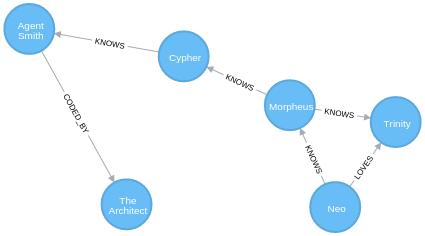
\includegraphics[width=0.8\textwidth]{img/matrix-graph}
\end{figure}
\begin{figure}[h!]
  \caption{Search Process for the automata in Figure \ref{fig:example-automata} }
  \label{fig:example-query-process}
  \centering
    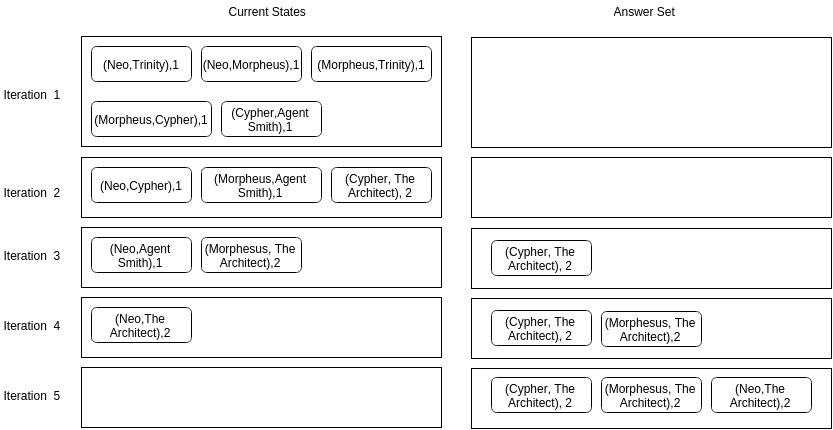
\includegraphics[width=1.0\textwidth]{img/Example-query-process}
\end{figure}
The search process is illustrated in Figure \ref{fig:example-query-process}:\\
For each state, the first pair such as $(Neo,Trinity)$ represents the start and end node in the graph, the second parameter like 1 or 2 represents the node position in automata. As the total number of visited states might be too large to show on this diagram, it's omitted here.
\subsection{Optimizations}
\subsubsection{Rare Labels}
Koschmieder and Leser propose a two-way BFS algorithm using rare labels in graph\cite{koschmieder2012regular}. The basic idea is to split the regular path query by rare labels and use them as fixed points to conduct two-way breadth first search. The rare labels would be determined by a user giving label frequencies.\\
The algorithm's advantages can be summarized as follows:
\begin{enumerate}
\item Rare labels occur much less in the graph, so we can reduce the search space when starting with rare labels.
\item For queries without matching pairs, we can achieve early stop by using rare labels.
\end{enumerate}
The algorithm can be done in 6 steps:
\begin{enumerate}
\item Locate all rare labels in the queries.
\item If there are more than one rare labels, find the paths between the first and second rare label, the second and third, etc.\ using a two-way search algorithm. If no path can be found in any of those search processes already, return an empty result set directly.
\item With the result from the previous step, find paths between the first and the last rare label.
\item From the first rare label, find all paths to the beginning of the regular expression.
\item From the last rare label, find all paths to the end of the regular expression.
\item Using the result from step 3, 4 and 5, generate all paths satisfying the regular expression and return the result set.
\end{enumerate}
For graphs with rare labels, the algorithm can speedup query evaluation by 90\%. However, if the graph or query contains no rare labels, the algorithm will still deteriorate to brute force search as introduced before. Furthermore, for many social network graphs, it's hard to define rare labels as there are only a limited number of labels and all of them are quite common.
\subsubsection{Path Index}
Peters' thesis work \cite{peters2015thesis} builds path indexes based on edge labels. A path index means for a specific path, or regular path expression, that we store all node pairs which meet the path. However, it's costly to store results for all possible paths for a graph, so Peter introduces the concept of k-path index, which means only paths of at most k steps will be stored.\\
For example, the 2-path index for example graph in Figure \ref{fig:example-matrix} would be:
\begin{table}[h!]
\def\arraystretch{1.5}
\centering
\caption{2-Path Index for MATRIX Graph}
\label{2-path-index}
\begin{tabular}{|l|m{20em}|}
\hline
Path            & Node pair                                                                \\
\hline
KNOWS           & (Neo,Morpheus), (Morpheus,Trinity), (Morpheus,Cypher), (Cypher,Agent Smith) \\
\hline
LOVES           & (Neo,Trinity)                                                            \\
\hline
CODED\_BY       & (Agent Smith, The Architect)                                             \\
\hline
KNOWS,KNOWS     & (Neo,Trinity),(Neo,Cypher),(Morpheus,Agent Smith)                             \\
\hline
KNOWS,CODED\_BY & (Cypher, The Architect)\\     
\hline
\end{tabular}
\end{table}
\\Peters adopts a similar approach with the rare label based algorithm and split the regular path query into smaller pieces according to histogram count of labels. Then for the sub-queries of relatively small size, path index could be looked up instead of searching graph, which saves time and I/O cost. Peters uses Postgres as back-end and elaborates carefully about the implementation details.\\
The limitation of path indexes shows when the query is long and the graph is dense, because then it might be very expensive to store the data structure. Moreover, in Peters' definition, the Kleene Star is not fully supported, instead lower and upper bound of the label occurrences is defined. 
\section{Distributed Evaluation of RPQ}
\subsubsection{Basic Definitions}
A distributed graph $DG$ is a graph whose nodes are partitioned into $m$ sets on $m$ sites. At each site $\alpha$, nodes and edges connecting them define a fragment $DG_\alpha$ of the distributed graph.\\
An edge $u\to v$ is called $cross-edge$ if $u$ and $v$ are stored on different sites.\\
For a cross-edge $u\to v$, $u$ is called output node, and $v$ is called input node.
\subsubsection{Algorithms}
The intuitive way to parallize RPQ evaluation is to query for each automata edge in parallel, then perform a multi-way join on the data. Again, to balance the search space and running time of algorithms, we can make use of fixed point strategy and search for sub-queries in parallel instead of searching for every automata edge at the same time. Dan Suciu has proposed an efficient algorithm\cite{suciu2002distributed} to evaluate RPQs on distributed graphs with distinguished properties as follows:
\begin{enumerate}
\item The number of communication steps is four, independent of the data and query.
\item The total amount of data exchanged during communication has the size of $O(n^2)+O(r)$, where 
$n$ denotes the number of cross-links in distributed database, $r$ the size of the result of the query.
\end{enumerate}
Dan's algorithm is improved by Tung, Nguyen-Van and Hu in \cite{tung2013efficient}, which decreases the data exchange size from $O(n^2)+O(r)$ to $O(|N|*|S|*|P|)$, where $N$ stands for number of input and output nodes, $S$ denotes number of nodes in automata, and $P$ is number of graph partitions.\\
Those two algorithms solve a more complex class of RPQ problems: they are trying to find all paths satisfying the given RPQ and only works on a rooted graph for semi-structure data such as XML. As the number of paths could be infinite in a cyclic graph and there might be multiple entry points for a graph, we will modify Dan's algorithm in section 4.
\section{Balanced Graph Partitioning}
As the data shuffled in distributed algorithms is related to graph properties such as number of input nodes or cross-edges, it's interesting to investigate how different partition strategies would affect the communication cost and try to optimize partition strategy for RPQ evaluation.\\
The balanced k-way graph partitioning can be defined as followed\cite{karypis1998multilevelk}: Given a graph $G = (V,E)$ with $|V| = n$, partition $V$ into $k$ subsets, $V_1,V_2,V_3,...,V_k$ such that $V_i\cap V_j=\emptyset$ for $i\neq j$, $|V_i|=n/k$ and the number of cross-edges is minimized. Here we require that the node size of each partition is the same as we want load balancing for query engine and using storage back-end that balance data over nodes such as Cassandra.\\
The direct computation of a good k-way partitioning is NP-hard problem\cite{karypis1998multilevel}, so the strategies in the survey below are all approximation algorithms.
\subsubsection{METIS}
METIS\cite{Karypis95metis} is a famous partitioning algorithm based on multilevel graph partitioning (MGP). MGP has three phases:
\begin{enumerate}
\item Shrink the graph to a smaller one by iteratively contracting edges and unifying nodes with four partitioning schemes in \cite{karypis1995multilevel}, which are:
    \begin{enumerate}
        \item Random Matching (RM): Each vertex coarsens with a random adjacent vertex.
        \item Heavy Edge Matching (HEM): Each vertex $u$ coarsens with an adjacent vertex $v$ such that the sum of edge weights $(u,v)$ is maximal.
        \item Light Edge Matching (LEM): Each vertex $u$ coarsens with an adjacent vertex $v$ such that the sum of edge weights $(u,v)$ is minimal.
        \item Heavy Clique Matching (HCM): Each vertex $u$ coarsens with an adjacent vertex $v$ such that the edge density is maximal. The motivation behind this scheme is to find highly connected components.
    \end{enumerate}
\item Partition the smallest graph after the graph is small enough to run a brute-force partitioning strategy inexpensively.
\item Bringing back the original graph by un-contracting edges and splitting the nodes. At the same time, do some local optimization to minimize edge cut.
\end{enumerate}
Although there are also other implementations based on MGP, such as KaFFPa\cite{sanders2011engineering} or \cite{soper2004combined}, in this project we select METIS as it has the fastest available parallel code and stable library. In this library, all of those four partitioning schemes mentioned above are applied and selected with smart policy according to the situation.
\subsubsection{JabeJa}
JabeJa\cite{rahimian2013jabeja} is a distributed balance partitioning algorithm which works in a different way from METIS: A k-way partitioning can be given with the help of a partition function $\pi$ which assigns a color from set \{1,2,3,...,k\} to each node. Let the number of neighboring nodes of node $p$ be $x_p$ and $x_p(c) = |N_p(c)|$ be the number of neighbors nodes of p with color $c$. The energy of the graph could be defined as followed:
$$E(G,\pi) = \sum_{p\in V} (x_p-x_p(\pi_p))$$
Then we can formulate the problem of optimal partitioning $\pi^*$ as followed:
$$\pi^* = \arg \min_{\pi} E(G,\pi)  $$ where $|V(c_1)|=|V(c_2)| $ for $\forall c_1,c_2 \in \{1,2,3,...,k\}$.\\
JabeJa is an iterative algorithm based on this model. For each iteration, every node will try to swap color with its neighbor and check if the swap makes the global energy smaller. The nodes only need to calculate the local result, which means they do not need global information to make a decision. There are several local search operators:
\begin{enumerate}
\item Local: every node selects its direct neighbors to swap color.
\item Random: every node select random nodes in the graph to swap color.
\item Hybrid: every node firstly applies the Local operator, then applies the Random operator after reaching the local optimum.
\end{enumerate}
Each time the nodes will swap color, the total number of nodes with each color will remain the same, which means the partition will keep balanced during the whole process. It's not possible to prove that JabeJa could get the optimal partition, but it could be easily customized to be based on other properties like input nodes number.
% \section{Graph Signature}
% Graph signature is a technique which encodes labels of each node into a bit-string. In gstore system\cite{zou2011gstore}, it's introduced for matching SPARQL queries with wildcards on large RDF graph. The basic definition will be as followed:\\
% Suppose the size of different labels in graph is $M$, then for every edge $e$, the edge signature $eSig(e)$ would be a bit-string where $(H(eLabel)\%M)$ -th bit set to '1', where $H(eLabel)$ is the hash-value of $eLabel$.\\
% Given a vertex $v$ from the graph, the vertex signature $vSig(v)$ is a bit-string constructed in following way:
% $$vSig(v)=eSig(e_1)|eSig(e_2)|......|eSig(e_n)$$
% where the $eSig(e_i)$ is the edge signature which starts from node v and "|" is the bitwise operation OR.\\ Given a graph $G$ and query $Q$, we can turn them into graph signature G* and query signature Q* by replacing each node and edge with the corresponding signature. For example, for MATRIX graph and a query $KNOWS\&LOVES$, the Q* and G* would be:\\
% \begin{figure}[h!]
%   \caption{Example of graph signature}
%   \label{fig:example-signature}
%   \centering
%     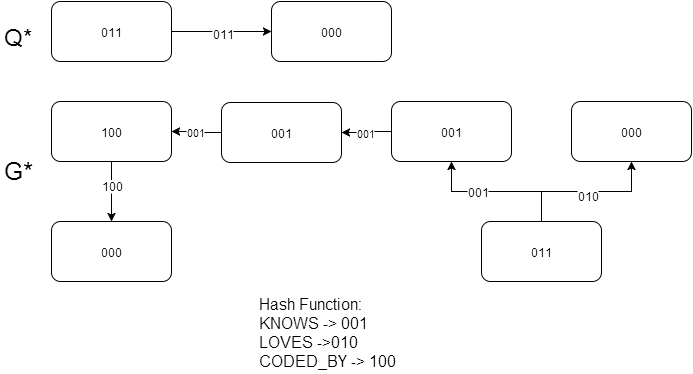
\includegraphics[width=0.8\textwidth]{img/signature-graph}
% \end{figure}
% \\Q* would be a sub-graph match for G* if and only if following conditions hold:\\
% \begin{enumerate}
% \item $vSig(v_i)\&vSig(u_i)=Vsig(v_i)$, i = 1,2,3,...,n, where '\&' is the bit-wise AND operator.
% \item If there is an edge from $v_i$ to $v_j$ in Q*, there is also an edge from $u_i$ to $u_j$ in G*.
% \end{enumerate}
% Although we cannot use this data signature in automata based RPQ evaluation directly, this technique could be useful while solving conjunctive regular path query. Comparing to Peter's index which is in depth-first way, the data signature is based on breadth-first principle. In section 5, we will illustrate how to build a vertex signature tree and combine it with distributed algorithm in order to accelerate CRPQ evaluation.e CRPQ evaluation.